\documentclass[fleqn]{article}

\usepackage{mydefs}
\usepackage{notes}
\usepackage{url}
\usepackage{amsmath}
\usepackage{graphicx}
\graphicspath{ {images/} }
\usepackage{verbatim}
\usepackage{subfig}
\usepackage[rightcaption]{sidecap}


\begin{document}
\lecture{Computer Vision}{Mini Project 04}
{Name:Abhay Doke {UID:29552668}}



\textbf{\huge 1.Pixel features}

For the pixel features I experimented with two methods where two sets of different normalizations were applied on the data. \newline
\vspace{5mm}

Method 1:
Making the data zero centered by mean-subtraction. Data is made zero centered by subtracting the mean across every individual feature in the data, and results in centering the cloud of data around the origin 
along every dimension.  
\begin{center}
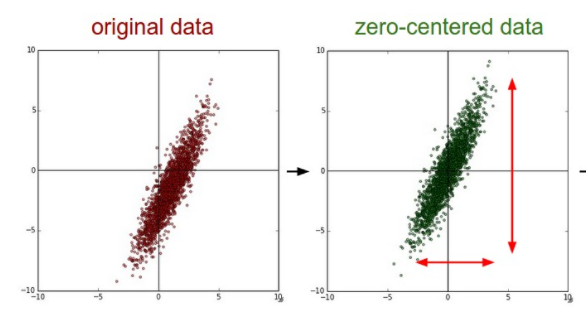
\includegraphics[width=0.8\textwidth]{zero_centered.png}
\end{center}

\vspace{10 mm}

Method 2:
Applying the L2-normalization followed by the square-root scaling.

Following are the accuracy result scores obtained by these two methods on the validation set and the test set.
\verbatiminput{pixelf.txt}

For the normal data, the L2-normalization followed by the square-root scaling performed the best with 87.6\% accuracy on the validation set. For the scaled data and the jittered data, mean-subtraction(method 1) worked better on 
both the validation as well as test dataset.  \newpage


\textbf{\huge 2.HoG features}

I used the 4 x 4 patches in the images to calculate the weighted histogram of oriented gradients. Image size is 28 x 28, so there are total 7 x 7 = 49 patches in each image.
Orientation values ranged from 0 - 360 degree and these values are binned into 18 bins viz. 0-20, 21-40, 41-60,...., 341-360.
So total number of features per image are 49*18 = 882.

Method 1: No normalization

Method 2: L2-normalization followed by the square-root scaling. Following results shows the validation set and the test set accuracies.
\verbatiminput{hogf.txt}

HoG features work very well for the normal data and the scaled data. L2-normalization followed by the square-root scaling worked better on all of the datasets as compared to the no normalization strategy.

\newpage

\textbf{\huge 3.LBP features}

For the LBP features I used two methods for calculating the LBP features.
The main observation of the LBP feature experiment was the exclusion of LBP feature with value 255 from the feature vector really improved the accuracies for all three datasets.
LBP feature with value 255 represents either all surrounding pixels are same or greater than the current pixel. Since most part of the images are either black or white, this feature
is not representing any significant information.   
Also the scaling the pixel values in the images do not alter the LBP accuracies i.e. the accuracies on the normal data and the scaled data with LBP features are almost the same.

Method 1: Calculating a single histogram of LBP features for the whole image. The resulting histogram size was 255 and hence the feature vector had 255 features.

Method 2: Each image was divided in two 4 parts and LBP feature histogram were calculated independently for all 4 patches. All of the four histograms were concatenated to obtain the final feature vector.
The resulting feature vector had 255*4 = 1020 features. 
\verbatiminput{lbpf.txt}

LBP features are representing the local patterns in images. Also they are invariant to the rotation and scaling to some extent. Hence the classification accuracy for the jittered data is better than other two feature types.

Below is the table showing the best accuracies achieved for each of the three datasets.
\verbatiminput{best.txt}

\vspace{10 mm}
Which feature works the best on normal digits? Why? --
HoG features works the best for the normal digits. HoG features captures the local gradient patterns over the many patches in the images. Digits have fixed gradient patterns over the different areas and if the data is not jittered like rotated or skewed these features will capture the most information from the data.

Which feature works the best on scaled digits? Why? --
Again data is scaled i.e. pixel values are scaled and as digits images are almost black and white, the local gradient patterns in the images still remains the same. Hence HoG features works the best followed by LBP features.

Which feature works the best on jittered digits? Why? --
In the jittered data images are translated. As images are translated we need an image descriptor which is invariant to small translations and LBP are the best features to handle such data.
LBP feature histogram remains the same if the image is translated. For example in an image number of pixels with value 10 are 100 and now if we translate the image, only pixel positions are shifted but the local patterns remains the same and hence number of pixels with value 10 will still be around 10. 
\newpage
Code for extractDigitFeatures.m

\verbatiminput{extractDigitFeatures.m}

For the LBP features, I tried 2-3 methods. One was from \url{http://www.springer.com/cda/content/document/cda_downloaddocument/9780857297471-c2.pdf?SGWID=0-0-45-1153741-p174122174}{ "Local Binary Patterns for Still Images"}. 
One which I tried was, Mappings of the LBP Labels: Uniform Patterns. This method generates LBP histogram with 9 bins only. Only LBP values representing uniform patterns such as Spot, Spot/Flat, Line End, Edge and Corner are kept as LBP features. 

\newpage

\textbf{\huge 4. Extension -- Random forest classifier}
\verbatiminput{randomf.txt}

Code of randomForest.m

\verbatiminput{randomForest.m}




\end{document}
